\documentclass[12pt]{article}

\usepackage[utf8]{inputenc}
\usepackage{geometry}
\geometry{margin=1in}
\usepackage{graphicx}
\usepackage{amsmath}
\usepackage{booktabs}
\usepackage{hyperref}
\usepackage{caption}
\usepackage{subcaption}
\usepackage{float}
\usepackage{listings}
\usepackage{xcolor}

\title{Incentives and COVID-19 Vaccinations Replication Project }
\author{Molly Marino}
\date{\today}

% Settings for code blocks
\lstset{
	basicstyle=\ttfamily\small,
	breaklines=true,
	frame=single,
	backgroundcolor=\color[RGB]{245,245,245},
	keywordstyle=\color{blue},
	commentstyle=\color{green!50!black},
	stringstyle=\color{red!50!brown},
	numbers=left,
	numberstyle=\tiny,
	stepnumber=1,
	numbersep=5pt
}

\begin{document}
	
	\maketitle
	\tableofcontents
	\newpage
	
	\section{Original Study}
The paper “Incentives Can Spur COVID-19 Vaccination Uptake” by Heike Klüver, Felix Hartmann, Macartan Humphreys, Ferdinand Geissler, and Johannes Giesecke examines whether policy incentives can increase individuals’ willingness to receive a COVID-19 vaccine. Written during the COVID-19 pandemic, the study addresses the problem of vaccine hesitancy, which threatened efforts to achieve high vaccination coverage and control the spread of the virus. The authors conducted a large survey experiment with approximately 20,500 participants in Germany, presenting respondents with different vaccination policy scenarios. These scenarios tested policies such as financial incentives, granting additional freedoms to vaccinated individuals, and making vaccines easier to access through local doctors. The results suggest that each of these policies can modestly increase willingness to vaccinate, particularly among individuals who are undecided rather than strongly opposed. The authors conclude that combining multiple incentives and improving access could be an effective strategy for policymakers seeking to increase vaccination rates. The study was necessary because there was little empirical evidence at the time on which policy tools could successfully encourage vaccine uptake during the pandemic.
	
	\section{Methods}
	The study examines data from a large survey experiment and applies regression analysis to evaluate how policy incentives influence individuals’ willingness to receive a COVID-19 vaccine. Participants were asked to consider a series of hypothetical vaccination scenarios that differed across several policy characteristics, such as financial incentives, access to vaccination through local physicians, and expanded freedoms for vaccinated individuals. These policy characteristics function as the key explanatory variables in the analysis. The dependent variable captures each respondent’s stated likelihood of choosing vaccination within the presented scenario. Linear regression models are then used to estimate the relationship between vaccination willingness and the randomly assigned policy attributes. This approach allows the authors to determine the marginal effect of each incentive on vaccination decisions.

	
	\section{Data}
	The analysis was carried out in R using R Markdown. The workflow was organised across three scripts. The first script, prep data, prepares and cleans the dataset used in the analysis. The second script, main results, estimates the baseline regression models and generates the main results tables. The third script, het effects, estimates heterogeneous treatment effects for different subgroups.
	
	All three scripts are compiled through a master document called index.Rmd using the rmarkdown::render() function. This runs each script in sequence and reproduces the full analysis pipeline.
	
\lstinputlisting[language=R, firstline=1, lastline=1]{Replication_Project.R}.
	
	\section{Original Model}
	
	Figures 1A, 1B, and 2ABC are based on regression and machine learning models estimating the effects of vaccination incentives. For Figure 1A, we implement first-differences regressions in which the change in an individual’s vaccination willingness between two vignettes is regressed on the differences in assigned treatments: negative incentives, financial incentives of 25 or 50 euros, and access to local doctors. We also estimate equivalent individual fixed-effects regressions using the stacked dataset, including a separate indicator for each individual to account for unobserved time-invariant characteristics. These regressions produce estimated coefficients representing the marginal effect of each incentive on vaccination probability.
	
	 Figure 1B uses these regression estimates to simulate predicted shares of the population vaccinated under counterfactual incentive combinations, including baseline (no incentives), local doctor plus freedom incentives, and all incentives applied simultaneously. Figure 2ABC uses a causal forest model to estimate heterogeneous treatment effects, predicting how each individual’s response to a given incentive varies with characteristics such as age, distance to vaccination centers, socio-economic status, and attitudinal measures. 
	 
	 Panel A reports which covariates are most predictive of treatment effect variation, Panel B shows how treatment effects differ across age groups and incentive types, and Panel C shows sensitivity to distance from vaccination centers. Together, these models quantify both average treatment effects and conditional individual-level effects of vaccination incentives.One limitation of the study is that the primary regressions assume additive effects of the different incentives. That is, the estimated coefficients reflect the average marginal effect of each incentive independently, without fully accounting for potential interactions between incentives or between incentives and individual characteristics.
	
\lstinputlisting[language=R, firstline=58, lastline=125]{Replication_Project.R}.

	
\subsection{Figure 1: Estimated Effects on Vaccination Probability}

Figure~\ref{fig:figure1} shows the estimated effects of different policy incentives on the probability of vaccination.

\begin{figure}[h]
	\centering
	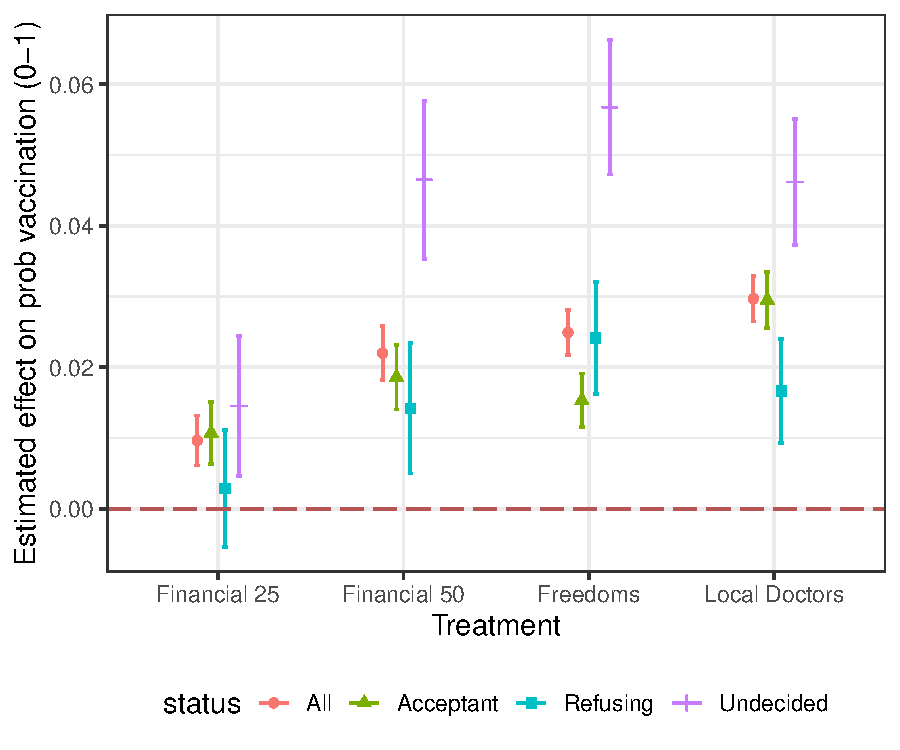
\includegraphics[width=0.9\textwidth]{figure_1A.pdf}
	\caption{Estimated effects on vaccination probability.}
	\label{fig:figure1}
\end{figure}

Figure 1 presents the estimated treatment effects of different incentives on the probability of vaccination. The regression estimates suggest that financial incentives increase vaccination intentions by roughly 3–5 percentage points, with the €50 incentive producing a slightly larger effect (around 0.04–0.05) than the €25 incentive (around 0.03–0.04). The freedom-related incentive generates an effect of approximately 0.02–0.03, while the local doctor endorsement increases the probability of vaccination by about 0.05–0.06, representing the largest effect among the treatments. The effects are heterogeneous across groups: individuals who are undecided exhibit the strongest response to incentives, while the treatment effects for individuals who are already refusing vaccination are close to zero. These results indicate that incentives mainly influence individuals who have not yet made a firm decision regarding vaccination.

Below is the R code used to generate Figure 1:

\lstinputlisting[language=R, firstline=3, lastline=13]{Replication_Project.R}.

\subsection{Figure 2: Estimated Effects on Vaccination Probability}
	

Figure 2 illustrates the predicted share of the population vaccinated under different policy scenarios. In the baseline scenario with no incentives, approximately 50--55\% of the population is vaccinated, with the remainder split between undecided and refusing individuals. Introducing local doctor messaging combined with freedom-related incentives increases the vaccinated share to roughly 60--65\%. When all incentives are implemented simultaneously, the predicted vaccination rate rises further to around 70--75\% of the population. The figure also shows that these increases primarily occur through a reduction in the share of undecided individuals, rather than a large shift among those strongly refusing vaccination.

\vspace{0.5cm}

\begin{center}
	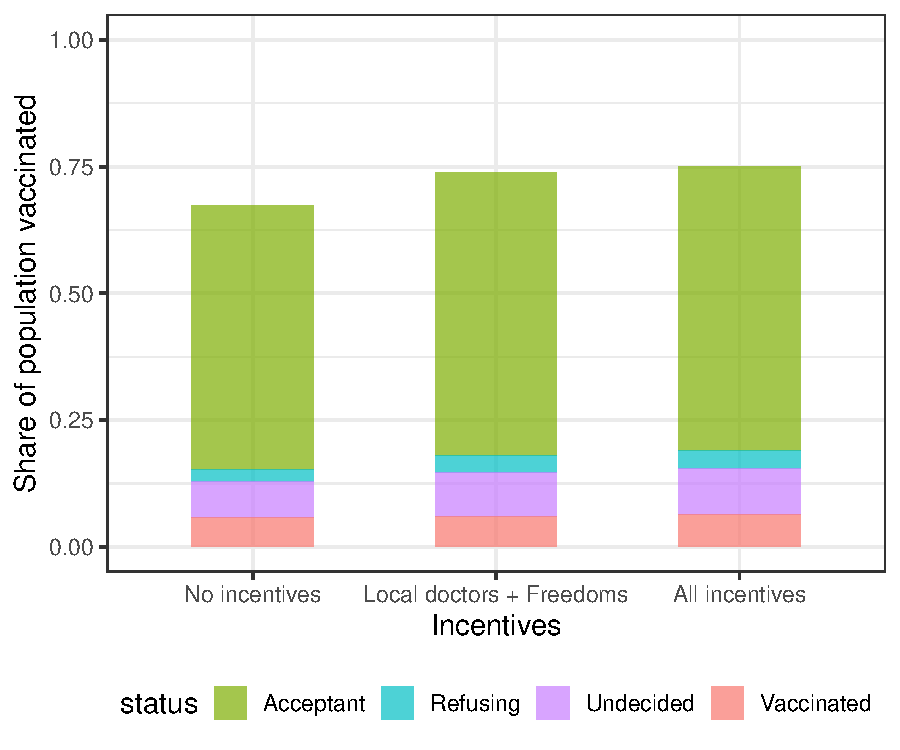
\includegraphics[width=0.9\textwidth]{figure_1B.pdf}
	
	\vspace{0.3cm}
	
	Figure 2: Share of population vaccinated under different policy scenarios.
\end{center}

\vspace{0.5cm}

R code for Figure 2:

\lstinputlisting[language=R, firstline=20, lastline=28]{Replication_Project.R}

	
\subsection{Figure 3: Heterogeneous Treatment Effects of Vaccination Incentives}

Figure 3 presents heterogeneous treatment effects of vaccination incentives estimated using a causal forest model. Panel A identifies the covariates most predictive of variation in treatment effects, with age, prior vaccine hesitancy, socio-economic indicators, and attitudinal measures, including trust in media and risk preferences, having the largest variable importance. Predicted conditional average treatment effects (CATEs) across individuals range from 0.01 to 0.12, with higher CATEs observed for older respondents for incentives designed to reduce logistical barriers. Panel B presents the interaction between age and incentive type among initially undecided respondents. The local doctor access incentive exhibits CATEs increasing with age, from approximately 0.05 in younger adults to 0.10 in older adults. Incentives based on enhanced freedoms exhibit decreasing CATEs with age, from approximately 0.08 in younger adults to 0.03 in older adults, whereas financial incentives produce CATEs of approximately 0.05 with minimal variation across age. Panel C reports CATEs as a function of geographic distance to vaccination centers. The local doctor incentive exhibits CATEs increasing with distance, ranging from 0.04 for respondents near centers to 0.09 for respondents farther away, consistent with reduced transaction costs; other incentive types display negligible sensitivity to distance. Overall, these results indicate that treatment effects are heterogeneous and moderated by individual characteristics and incentive type.

\vspace{0.5cm}

\begin{center}
	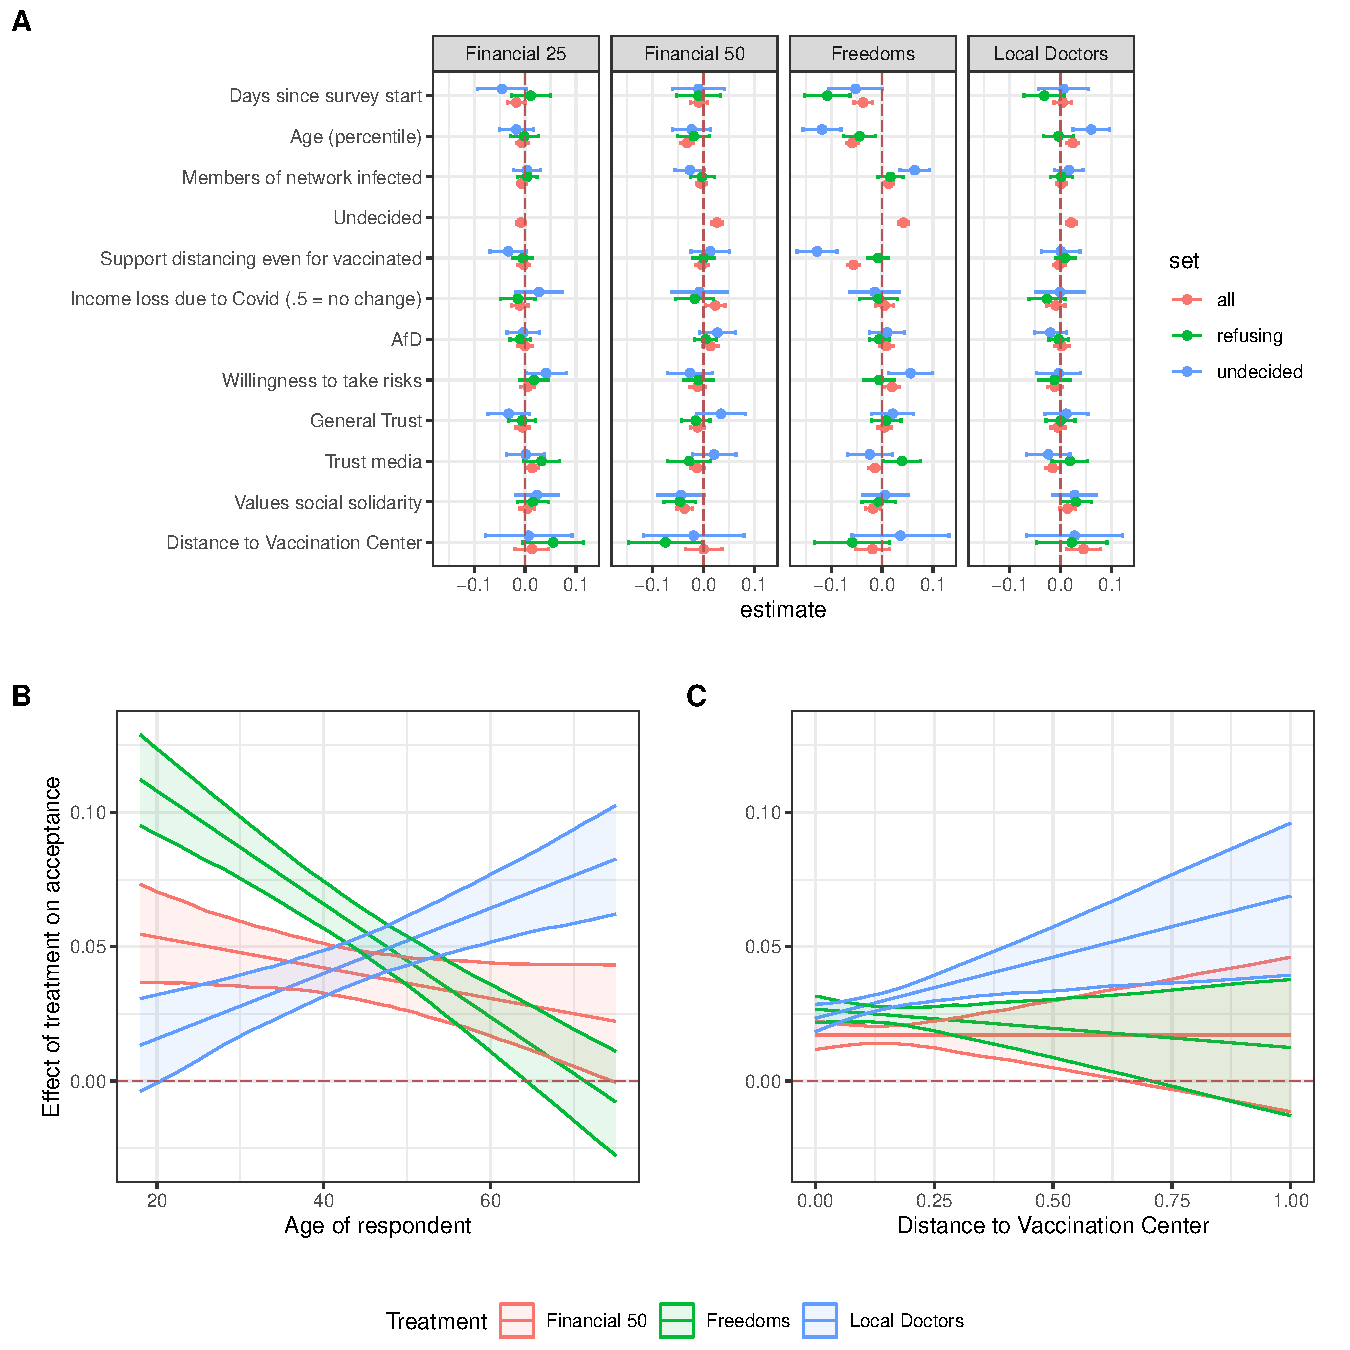
\includegraphics[width=0.9\textwidth]{fig_2_ABC.pdf}
	
	\vspace{0.3cm}
	
	Figure 3: Estimated heterogeneous treatment effects of vaccination incentives across individual characteristics.
\end{center}

\vspace{0.5cm}

R code for Figure 3:

\lstinputlisting[language=R, firstline=37, lastline=52]{Replication_Project.R}
\section{Modifications to Study}

To examine heterogeneity in treatment effects, we modified the original regression by including interaction terms between each treatment and normalized age (\texttt{age2}). The original model assumed additive effects, implying that each incentive had the same impact on vaccination probability for all respondents. By including interactions, the model estimates both the average effect of each treatment and how the effect changes with age. Formally, the model is specified as 
\[
\text{outcome\_diff} \sim \text{treatment} + \text{treatment} \times \text{age2},
\] 
where the coefficient on the interaction term measures the additional change in the treatment effect per unit increase in age. Using this model, we calculated predicted treatment effects across the age distribution. For example, for the Freedoms incentive, the predicted increase in vaccination probability is approximately 0.02 for younger respondents and rises to around 0.08 for older respondents, with 95 percent confidence intervals excluding zero, indicating statistical significance. Similar patterns are observed for the financial incentives, while the local doctor incentive shows little variation with age. These results demonstrate that the effect of vaccination incentives is not uniform across the population and that older respondents respond more strongly to certain treatments.

\lstinputlisting[language=R, firstline=131, lastline=160]{Replication_Project.R}

\begin{figure}[H]
	\centering
	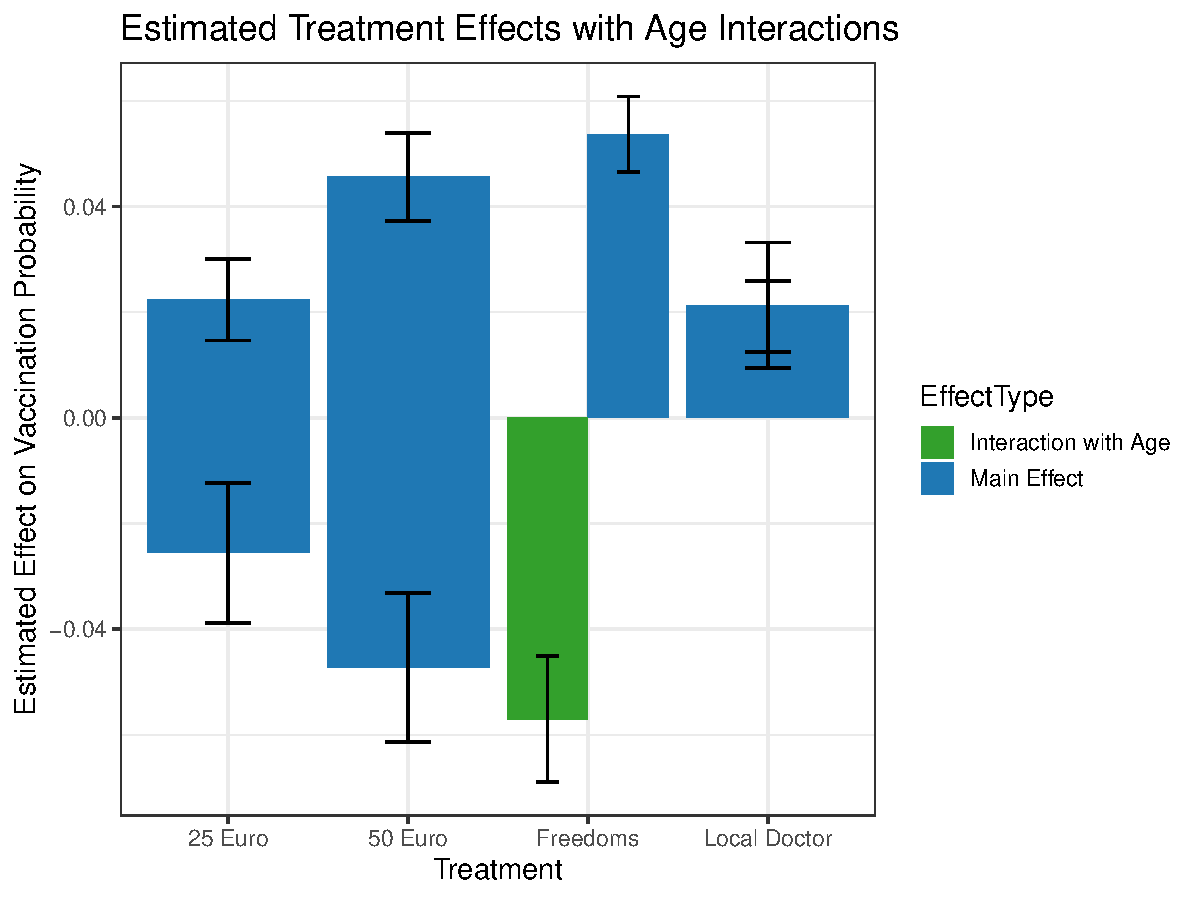
\includegraphics[width=0.8\textwidth]{Figure_Interaction_Age.pdf}
	\caption*{Figure 4: Predicted treatment effects across age groups.}
	\label{fig:interaction_age}
\end{figure}
\end{document}